\begin{frame}\frametitle{Mapping Rules}

% The underlying entity of every GraphQL schema is a type. Thereby there are six types of named type definitions and two wrapping types~\cite{gql-spec}. 
\footnotesize
\begin{itemize}

  \li{Positional Constructors} GraphQL fields must always have names~\cite{gql-spec}. 
  That why we assume that a constructor without field selectors is enumerated like an array.
  
  \importHS{positional-cons}{Positional Constructors}

  \li{Unit Type} The unit type indicates the absence of a specific value and serves as a placeholder when no other value exists or is needed~\cite{fsharp-unit}. GraphQL does not provide it~\cite{gql-spec}. 

  \importGQL{unit-type}{GraphQL Unit Type Definition}

\end{itemize}
\end{frame}


\begin{frame}\frametitle{Architecture Overview}
  \begin{enumerate} 
  
    \footnotesize

    \li{morpheus-graphql-core} low level functionalities and common types, such as  parsing, pretty-printing, validation.
  
    \li{morpheus-graphql-client} enables type-safe client queries. It generates the query and response types on valid queries but throws a compilation error on the invalid query.
  
    \li{morpheus-graphql-app} creates and executes GraphQL applications (called \expr{Apps}) based on schema and query documents.
    
    \li{morpheus-graphql-subscriptions}  creates WebSockets servers based on \expr{Apps}. It is independent of the server package and accepts any \expr{App} derived from an arbitrary server.
  
    \li{morpheus-graphql} derives executable \expr{Apps} from native Haskell types by mapping them to GraphQL representations. 
  
  \end{enumerate}

  % %!TEX root = ../../main.tex

\begin{figure}
\caption{
    Dependency Graph of the Morpheus GraphQL Packages
    \label{fig:dependency-graph}
    }
\begin{center}
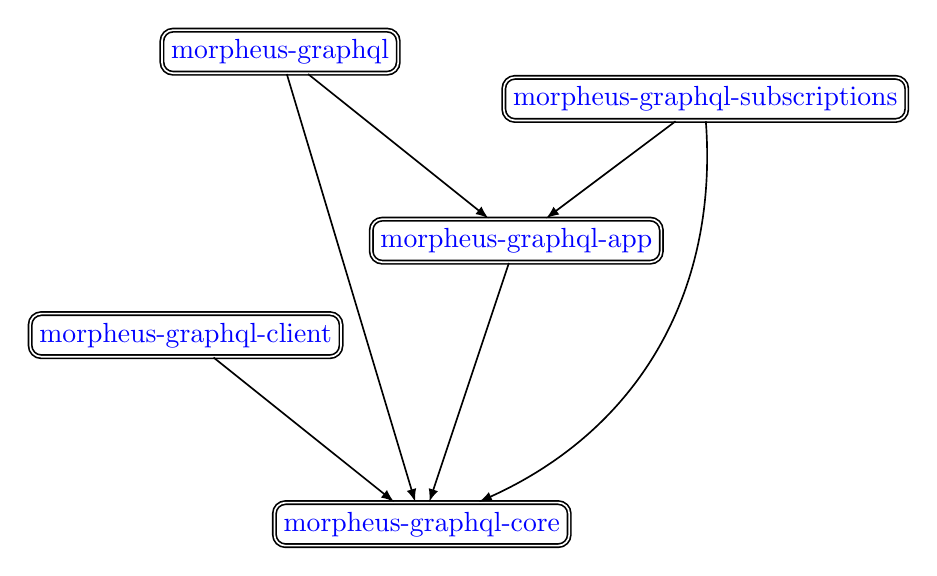
\begin{tikzpicture}[
        scale=.6,
        auto=left,
        -latex ,
        auto ,
        node distance =2 cm and 2cm ,
        % on grid ,
        semithick ,
        package/.style ={ fill=red!20,draw,double,rounded corners ,top color =white ,draw , text=blue , minimum width =1 cm},
    ] 
    \node[package] (core) at (10,0) {morpheus-graphql-core};
    \node[package] (client) at (5,4)  {morpheus-graphql-client};
    \node[package] (app) at (12,6)  {morpheus-graphql-app};
    \node[package] (server) at (7,10)  {morpheus-graphql};
    \node[package] (subs) at (16,9) {morpheus-graphql-subscriptions};
  
    \path (client) edge (core);
    \path (app)  edge (core);
    \path (server)  edge  (core);
    \path (server)  edge  (app);
    \path (subs)  edge  (app);
    \path 
        (subs) 
            edge [bend left =35] 
        (core);  

\end{tikzpicture}
\end{center}
\end{figure}
  
\end{frame}


\begin{frame}\frametitle{Datatype-Generic Programming}
    
  Datatype-generic programming enables writing single functions that address various cases and types.~\cite{derivable-type-classes}. 
  It increases program reliability, reduces code duplication, while guaranteeing safety~\cite{datatype-generic-programming,optimizing-generics}.
  
  \importHS{generics}{Generic Deriving}
      
  The generic derivation represents all types and values by generic representation types. The user can convert any types to their generic representation, operate on them, and convert them back to their original types~\cite{optimizing-generics, ghc-generics}.
  
  \end{frame}

\begin{frame}\frametitle{Monads}

Haskell abstracts side effects with monads. monads are formed by a type constructor \expr{M} and a pair of functions, \expr{return} and \expr{>>=}~\cite{history-of-haskell,essence-of-fp}. The type \expr{M a} is a computation that returns a value of type \expr{a} and possibly performs some side effects~\cite{history-of-haskell}. The purpose of \expr{return} and \expr{>>=} is to push a value into computation and to evaluate a computation, yielding a value~\cite{essence-of-fp}.

Since the monad allows the compiler to determine impure and pure operations, the Haskell language can use specific optimizations. However, the developer still has the freedom to define their execution order~\cite{history-of-haskell}.

\end{frame}

\begin{frame}\frametitle{Determining GraphQL Types in Haskell}
Compiler applies the following rules with a given execution order to achieve deterministic derivation.
\begin{enumerate}
  \li{Scalar, Wrapper, Interface} Derive scalar, wrapper, interface if the type has explicitly specified associated kinds. 
  \li{Field Arguments} Derive field arguments if the type is used as an argument of the object field. 
  \li{Enum} Derive enum if all data type constructors are empty.
  \li{Object} Derive object if the type has a single non-empty constructor, and its parent \footnote{Type A is the parent type of type B if it has a field that refers to type B} is Object or Union. 
  \li{InputObject} Derive input object if the type has a single non-empty constructor, and its parent is InputObject or Field Arguments.
  \li{Union} Derive Union if the type has multiple constructors and its parent is Object or Union.
  \li{Fail} All other types are not supported.
\end{enumerate}
\end{frame}
